\documentclass[]{beamer}

\usepackage{fontspec} 
% \usepackage{lsp-makros}
\useoutertheme{lsp}

\usepackage{lsptitle}

\def\two@digits#1{\ifnum#1<10 0\fi\number#1}
\def\mytoday{\two@digits{\number\day}.\two@digits{\number\month}.\number\year}


\usepackage{xspace,multicol}
\newcommand{\latex}{\LaTeX\xspace}
\usepackage{tikz}


\newcounter{lastpagemainpart}
\footnotesep0pt
\renewcommand{\footnoterule}{}
\usefootnotetemplate{
  \noindent
  \insertfootnotemark\insertfootnotetext}

\let\beamerfn=\footnote
\renewcommand{\footnote}[1]{%
\let\oldfnsize=\footnotesize%
\let\footnotesize=\tiny%
\beamerfn<\thebeamerpauses->{#1}%
\let\footnotesize=\oldfnsize}


\date{\today}

\usepackage{eurosym}  
 
\renewcommand{\centerline}[1]{\hfill#1\hfill\hfill\mbox{}}
\newcommand{\highlight}{\mdseries\color{red!80!black}}

\title{Accès libre -- Open Access\\For whom -- pour qui?}
% \institute{FU Berlin}
\author[Nordhoff]{Sebastian Nordhoff}
\date{FieldLing, Paris, 2022-09-09}


\begin{document}
\lspbeamertitle

\frame{
\frametitle{Sebastian Nordhoff}
%   \includegraphics[height=.2\textheight]{./path/to/graphicsfile}
  \begin{itemize}
    \item PhD 2009 \textit{A grammar of Upcountry Sri Lanka Malay}
    \item 3 edited volumes, about 30 research articles
    \item 2009-2012 Glottolog.org at the Max Planck Institute for Evolutionary Anthropology
    \item advocate for Open Source, Open Access, Open Data, Open Everything 
    \item since 2014 coordinator for Language Science Press
    \item involved in the publication of 180+ books since 2014
  \end{itemize}
}

\frame{
\frametitle{Language Science Press}
%   \includegraphics[height=.2\textheight]{./path/to/graphicsfile}
  \begin{itemize}
    \item  scholar-owned, community-based publisher 
    \item Open Access
    \item free to read 
    \item free to publish 
    \item 30 series
    \item 30 books a year (monographs and edited volumes)
    \item Publisher of several award-winning books
    \begin{itemize}
      \item     \textbf{Pāṇini award} (Grimm, Nadine. 2021. \textit{A Grammar of Gyeli}),
     \item \textbf{Greenberg award} (Easterday, Shelece. 2020. \textit{Highly complex syllable structure})
    \item  \textbf{von der Gabelentz Award} (Döhler, Christian. 2018. \textit{A grammar of Komnzo})
    \end{itemize}
    \end{itemize}
}

\frame{
\frametitle{Language Science Press}
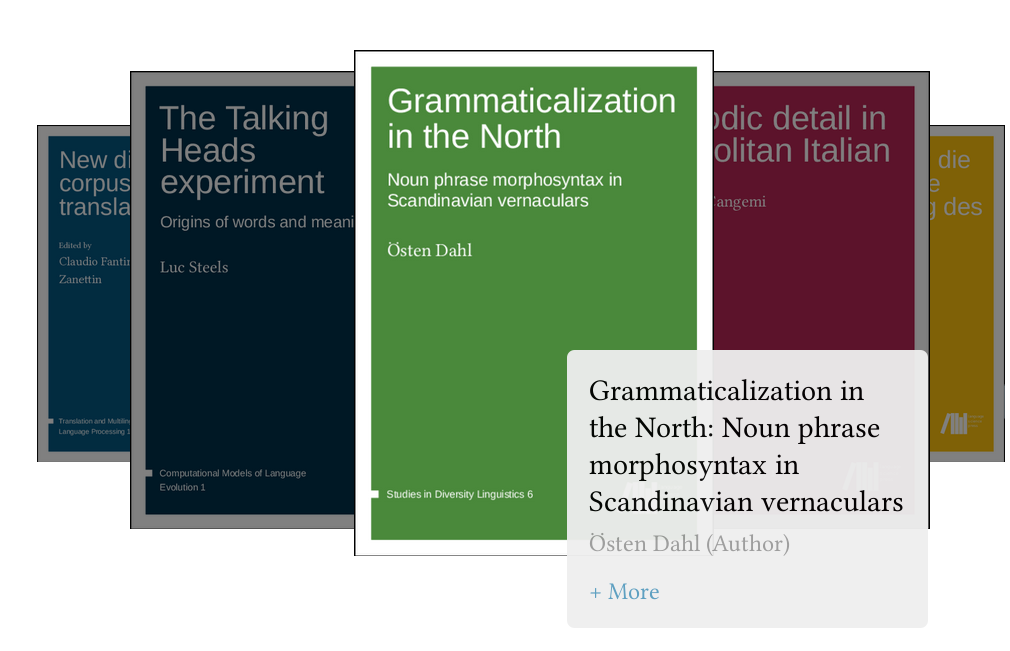
\includegraphics[height=\textheight]{catalog.png}
}
% 
% \frame{
% \frametitle{Production of a book:\\ traditional model}
% %   \includegraphics[height=.2\textheight]{./path/to/graphicsfile}
%   \begin{enumerate}
%     \item inquiry
% 	\item book proposal
% 	\item proposal approval
% 	\item contract
% 	\item first submission
% 	\item review
% 	\item first decision
% 	\item revision
% 	\item final decision
% 	\item copyediting
% 	\item first proofs
% 	\item typesetting
% 	\item final proofs
%   \end{enumerate}
% }


\frame{
\frametitle{Tenets}
%   \includegraphics[height=.2\textheight]{./path/to/graphicsfile}
  \begin{itemize}
\item    We want to share our knowledge
\item     We want to arrive at new findings regarding human language(s) and share these findings with everyone interested
\begin{itemize}
  \item         other researchers
  \item       speakers
  \item       general public
\end{itemize}
  \item   How can we achieve these goals?
 \end{itemize}
}

\frame{
\frametitle{The FAIR principles}
%   \includegraphics[height=.2\textheight]{./path/to/graphicsfile}
  \begin{itemize}
    \item  \textbf{F}indable
    \item \textbf{A}ccessible
    \item \textbf{I}nteroperable
    \item \textbf{R}eusable
  \end{itemize}
}

\frame{
\frametitle{Findable}
%   \includegraphics[height=.2\textheight]{./path/to/graphicsfile}
  \begin{itemize}
    \item  Use repositories
    \begin{itemize}
      \item do not use www.myname.com/thesis.pdf
      \item try to use domain specific repositories
    \end{itemize}
    \item Fill in all metadata fields as far as possible
    \begin{itemize}
      \item author name, title, subject, languages, coordinates
    \end{itemize}
  \end{itemize}
}

\frame{
\frametitle{Accessible}
  \begin{itemize}
    \item  no paywalls
    \item no complicated access protocols

  
\includegraphics[height=.5\textheight]{stefanmuellerpaywall.png}
  \end{itemize}
}

\frame{
\frametitle{Interoperable}
%   \includegraphics[height=.2\textheight]{./path/to/graphicsfile}
\begin{itemize}
    \item Documents come in different formats (pdf, jpg, mov)
    \item For your work to be accessible to others, you should use fileformats which are
    \begin{itemize}
    \item  standardized
    \begin{itemize}
      \item a skilled and motivated person should be able to write an application to read and write the format
      \item otherwise, your file risks ending up in a data graveyard
    \end{itemize}
    \item   open
    \begin{itemize}
      \item royalty-free
    \end{itemize}
    \item   suited for tasks
    \begin{itemize}
      \item eg, do not use jpg for texts
    \end{itemize}
    \end{itemize}
    \item \url{https://en.wikipedia.org/wiki/List_of_open_formats}
  \end{itemize}

}

\frame{
\frametitle{Sample table}
\begin{itemize}
  \item what an easy table looks like to humans
\end{itemize}

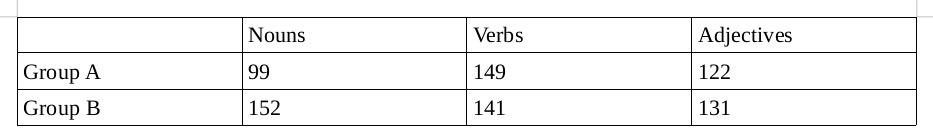
\includegraphics[height=.2\textheight]{sampletable_oo.png}

\begin{itemize}
  \item what an easy table looks like to computers
\only<2>{\textbf{png}:\\ 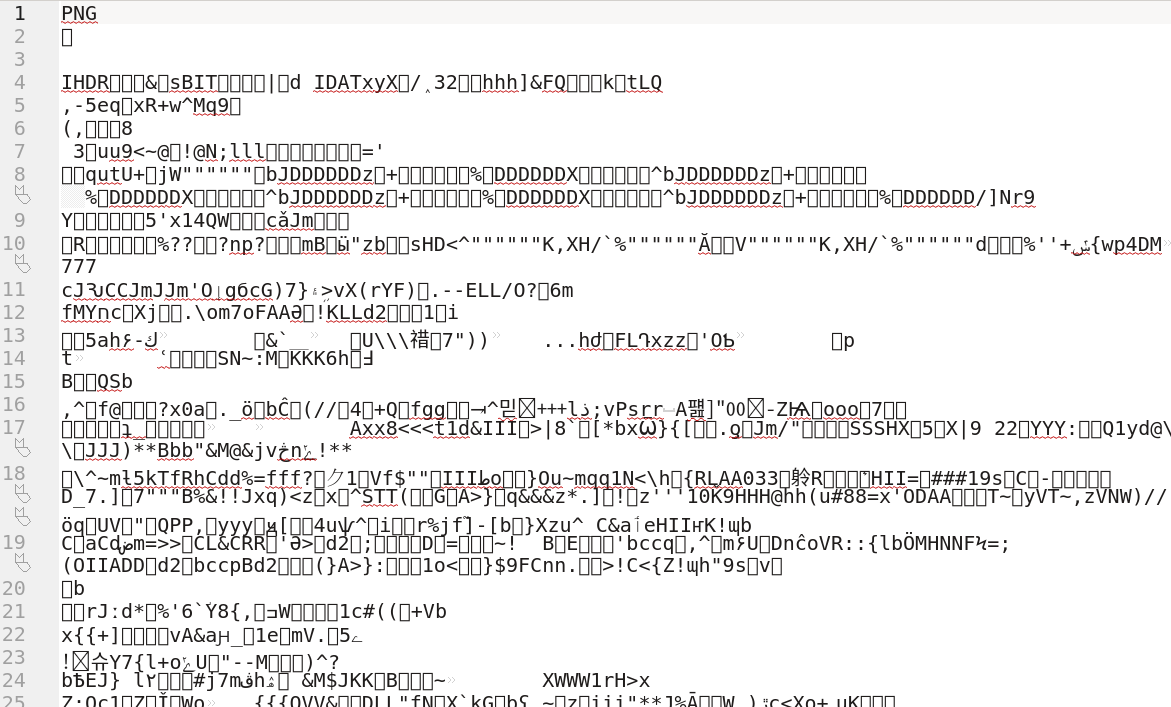
\includegraphics[height=4cm]{sampletable_png.png}}
\only<3>{\textbf{pdf}:\\ 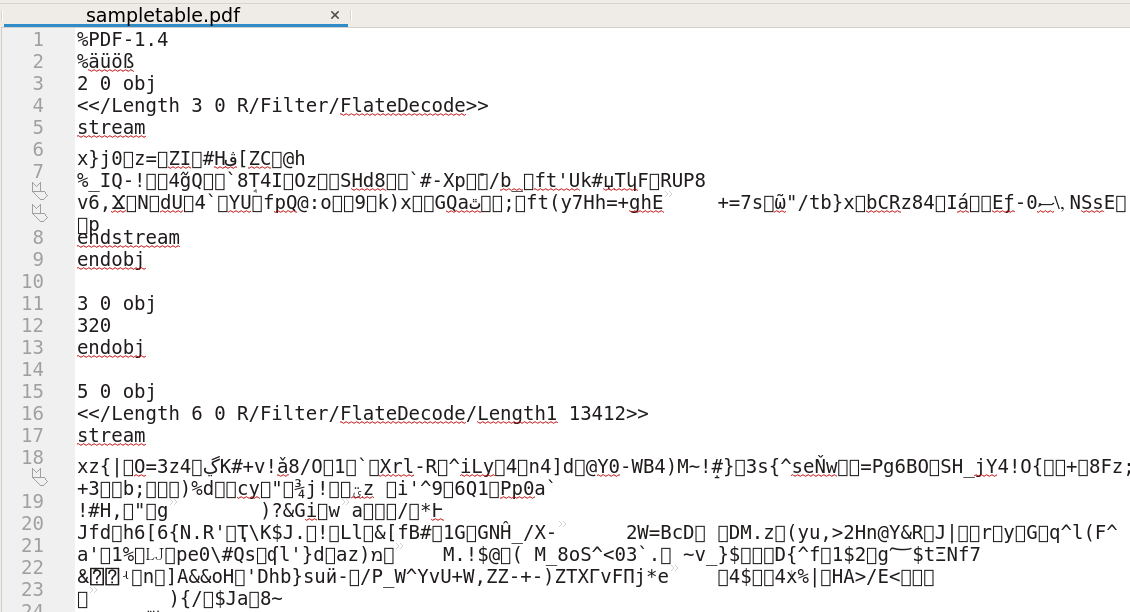
\includegraphics[height=4cm]{sampletable_pdf.png}}
\only<4>{\textbf{LibreOffice XML}:\\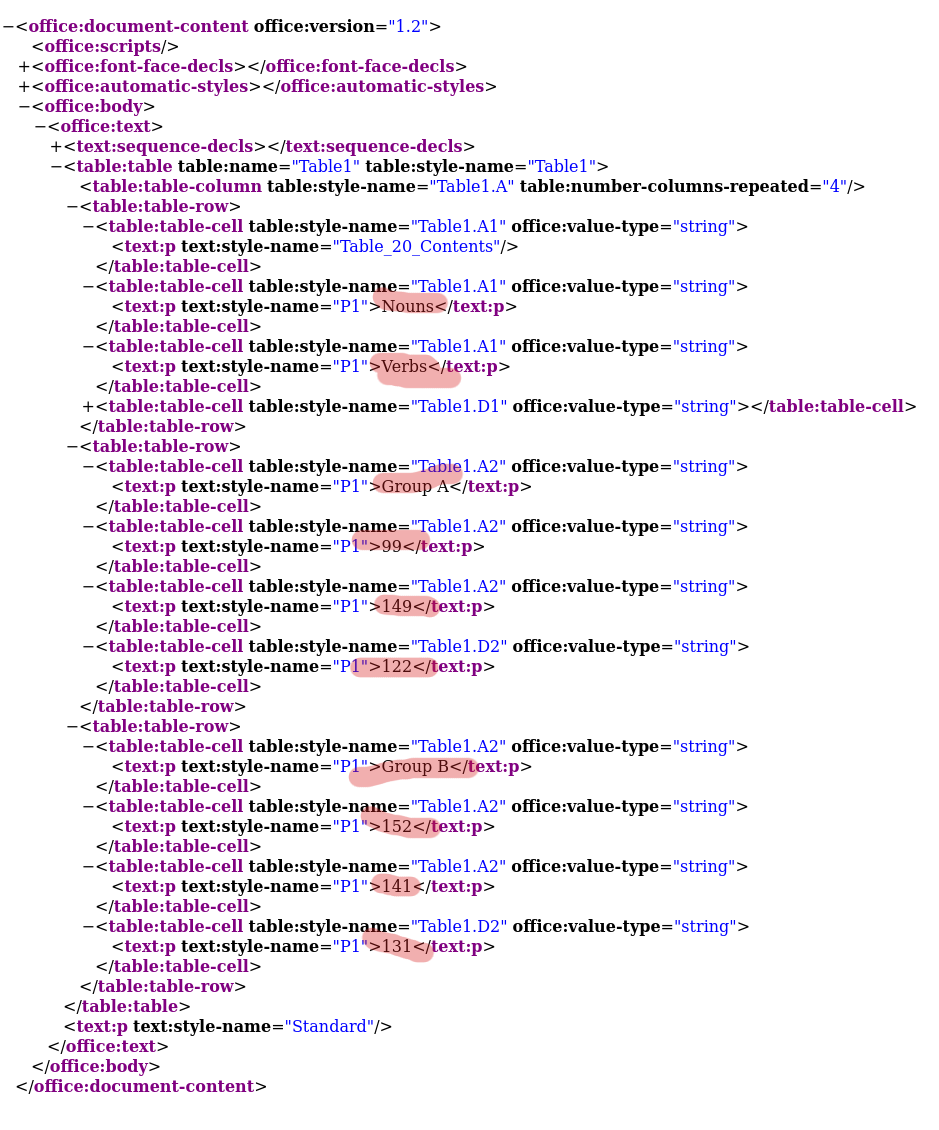
\includegraphics[height=8cm]{sampletable_xml.png}}
\only<5>{\textbf{csv}:\\ 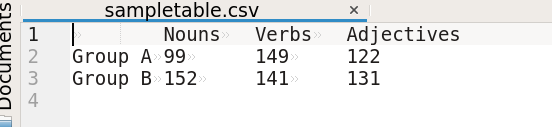
\includegraphics[height=3cm]{sampletable_csv.png}}
\end{itemize}
}

 \frame{
\frametitle{Reusable}
%   \includegraphics[height=.2\textheight]{./path/to/graphicsfile}
  \begin{itemize}
    \item  who wants to reuse your data?
    \begin{itemize}
      \item unlikely: Disney, Walmart, Amazon
      \item likely: researchers, linguistic blog, language schools
    \end{itemize}
    \item choose a suitable license to allow reuse with attribution
  \end{itemize}
}

\frame{
\frametitle{Licenses}
%   \includegraphics[height=.2\textheight]{./path/to/graphicsfile}
  \begin{itemize}
    \item  Use a Creative Commons License
    \item \textbf{good:} CC-BY, CC-BY-SA
    \item \textbf{bad:} CC-BY-ND (no translations, no excerpts, no cropping, no recomposition)
    \item \textbf{very bad:} CC-BY-NC: no blogs with ads, no language schools, no exhibitions with fees.
    \item \textbf{the worst:} CC-BY-NC-ND
  \end{itemize}
  \url{https://www.wikimedia.de/w/images.homepage/1/15/CC-NC_Leitfaden_2013_engl.pdf}
}

 \frame{
\frametitle{The Bad Guys: plagiarists}
%   \includegraphics[height=.2\textheight]{./path/to/graphicsfile}
  \begin{itemize}
    \item Plagiarists
    \begin{itemize}
        \item Plagiarists take their work and pretend it is theirs
        \item They do this regardless of copyright status
        \item The punishment for plagiarism is exclusion from the scientific community, not some civil lawsuit
    \end{itemize}
  \end{itemize}
}

 \frame{
\frametitle{The Bad Guys: Pirates}
%   \includegraphics[height=.2\textheight]{./path/to/graphicsfile}
  \begin{itemize}
    \item Pirates
    \begin{itemize}
      \item Pirates make your work available (possibly for a fee) without your consent
      \item They do this regardless of copyright status
      \item Every copyrighted movie, every copyrighted song, and every copyrighted trade book can be found on pirate sites on the internet
      \item The idea that a pirate would somehow be interested in legal provisions is very funny.
    \end{itemize}

    \item Both plagiarists and pirates know that what they do is illegal
    \item Piracy is in general not a big deal in science, but plagiarism can be.
    \item \textbf{BUT: restrictive licenses restrict the good guys}  (language schools, blogs), not the bad guys
  \end{itemize}
}

\frame{
\frametitle{Data, code, text}
%   \includegraphics[height=.2\textheight]{./path/to/graphicsfile}
\begin{columns}
  \column{6cm}
  \begin{itemize}
    \item  Clearly separate your \textbf{raw data}, the \textbf{code} you use to analyze the data, and the \textbf{write-up}
    \item Different repositories exist for each
    \item the image to the right had the data hard-wired into the code.
    \item The author replaced the data in the script for each diagram (there are 100)
    \item $\to$ It was not possible to recreate the image with different colours
  \end{itemize}
  \column{4cm}
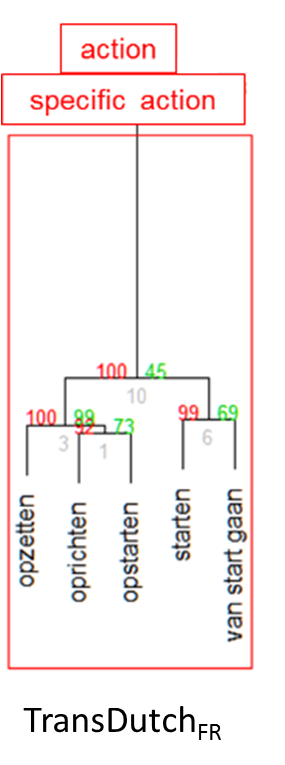
\includegraphics[height=1.2\textheight]{pngR.png}
\end{columns}
}

\frame{
\frametitle{Where to put your FAIR data? Repositories}
%   \includegraphics[height=.2\textheight]{./path/to/graphicsfile}
  \begin{itemize}
    \item Repositories collect documents and research data 
      \begin{itemize}
        \item \textbf{discipline-specific} or \textbf{general purpose}
        \item \textbf{preprint} or \textbf{postprint} 
        \item \textbf{text} or \textbf{data} or \textbf{code}
      \end{itemize}
  \end{itemize}
}

\frame{
\frametitle{Code repositories}
%   \includegraphics[height=.2\textheight]{./path/to/graphicsfile}
  \begin{itemize}
    \item  GitHub\\ 
\includegraphics[height=2cm]{github1.png}
    \item  GitLab\\ 
\includegraphics[height=2cm]{gitlab.png}
  \end{itemize}
}

\frame{
\frametitle{GitHub repositories}
  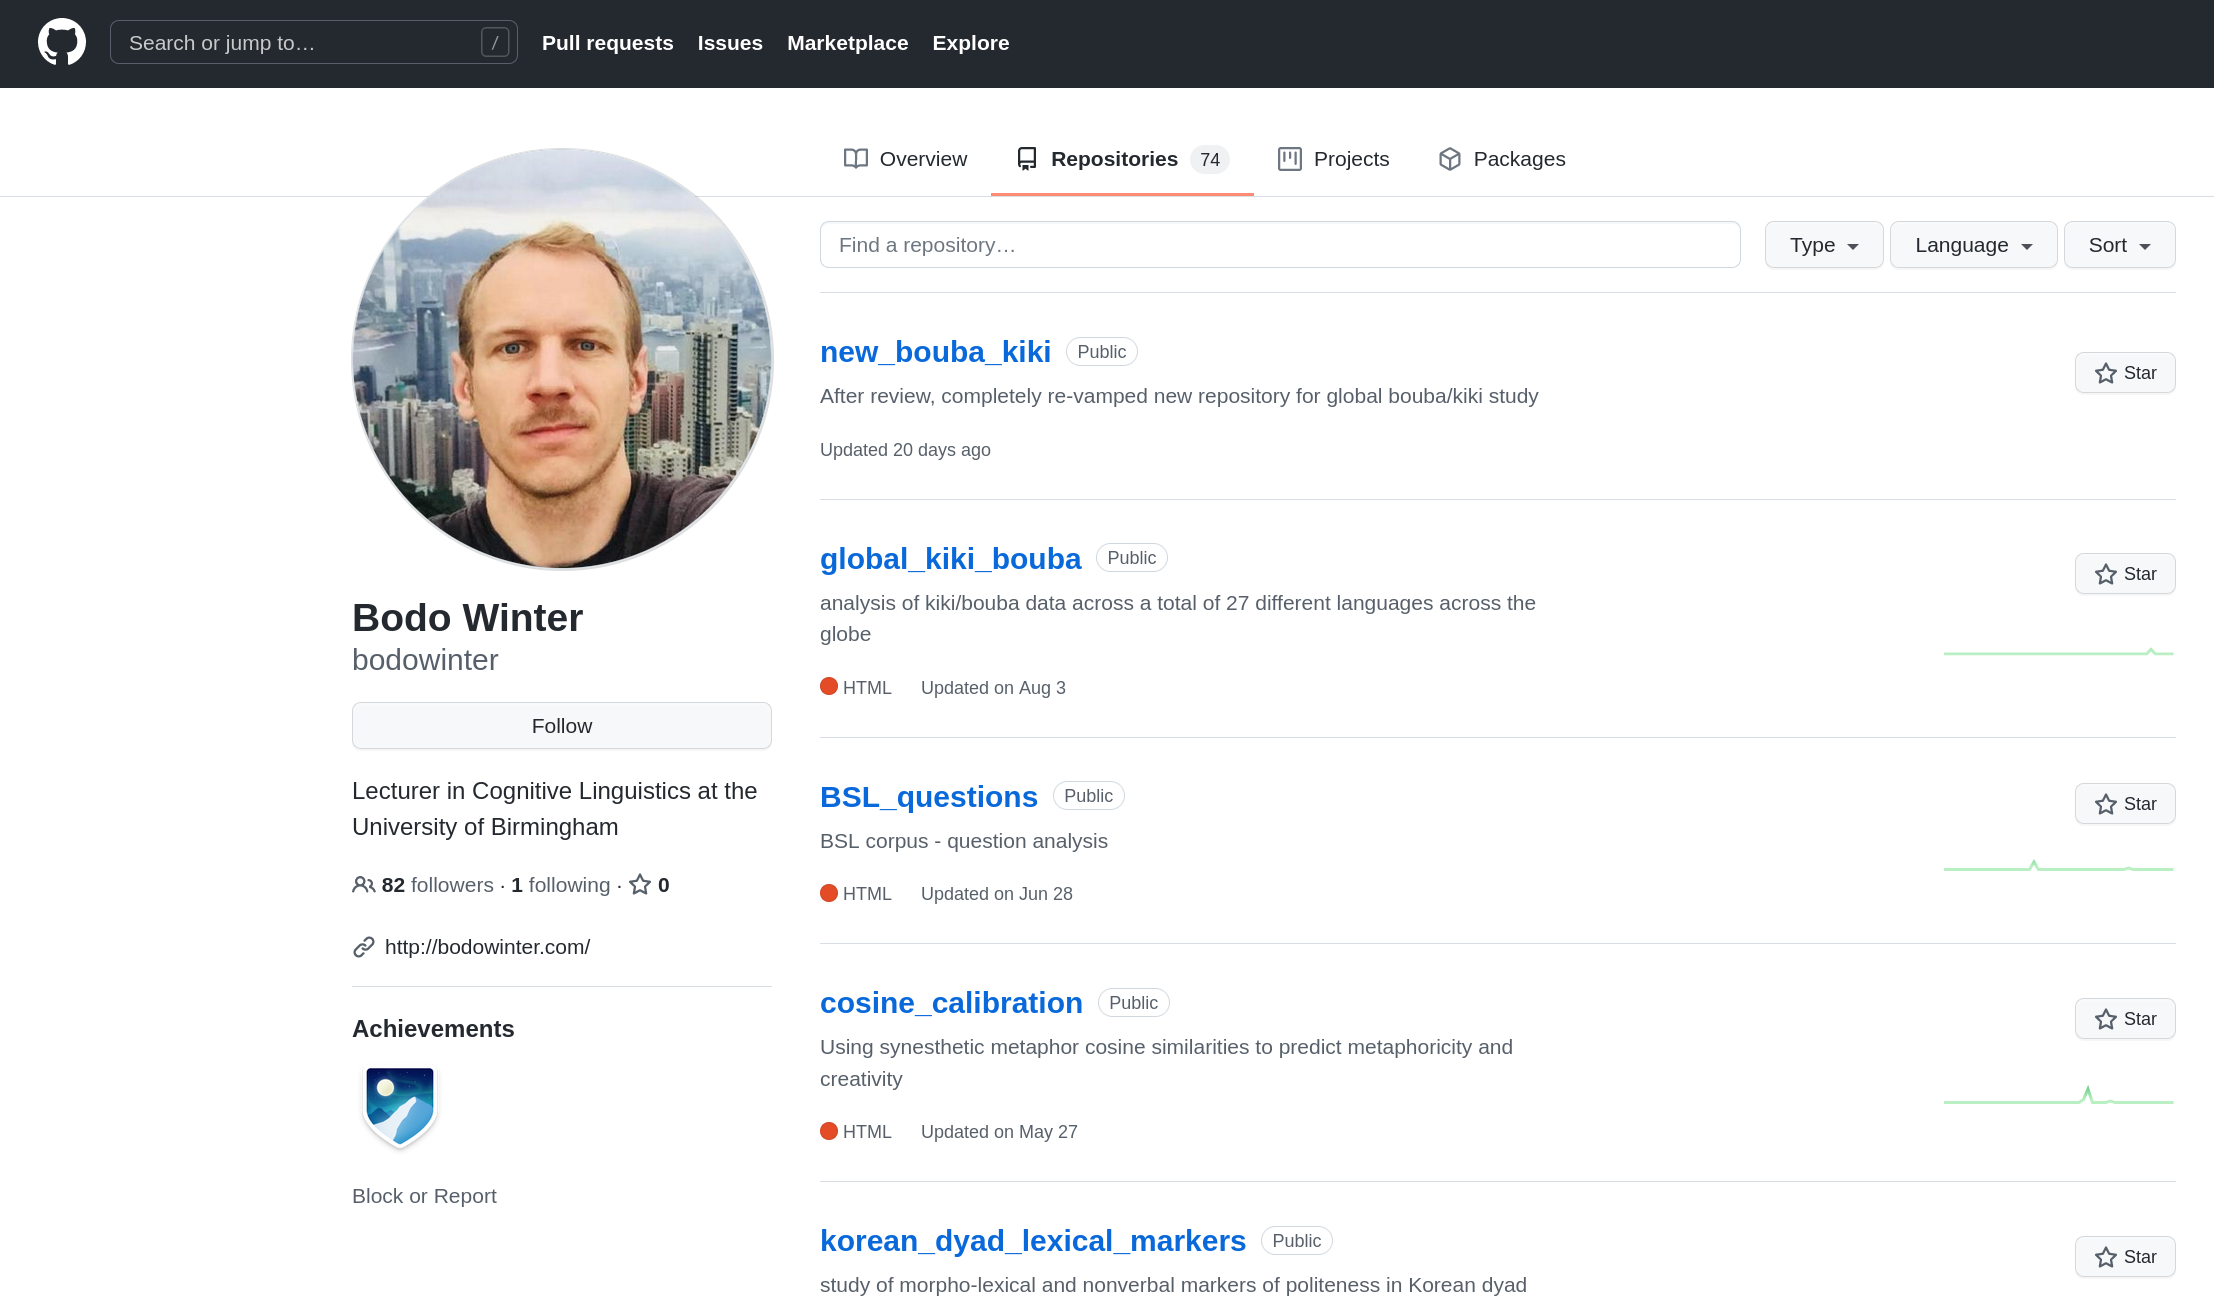
\includegraphics[height=\textheight]{bodowinter.png}
}

\frame{
\frametitle{Multimedia}
%   \includegraphics[height=.2\textheight]{./path/to/graphicsfile}
  \begin{itemize}
    \item  Paradisec
    \item ELAR
    \item AILLA
    \item TLA Nijmegen
  \end{itemize}
}

\frame{
\frametitle{Paradisec}
  \hspace*{-.5cm}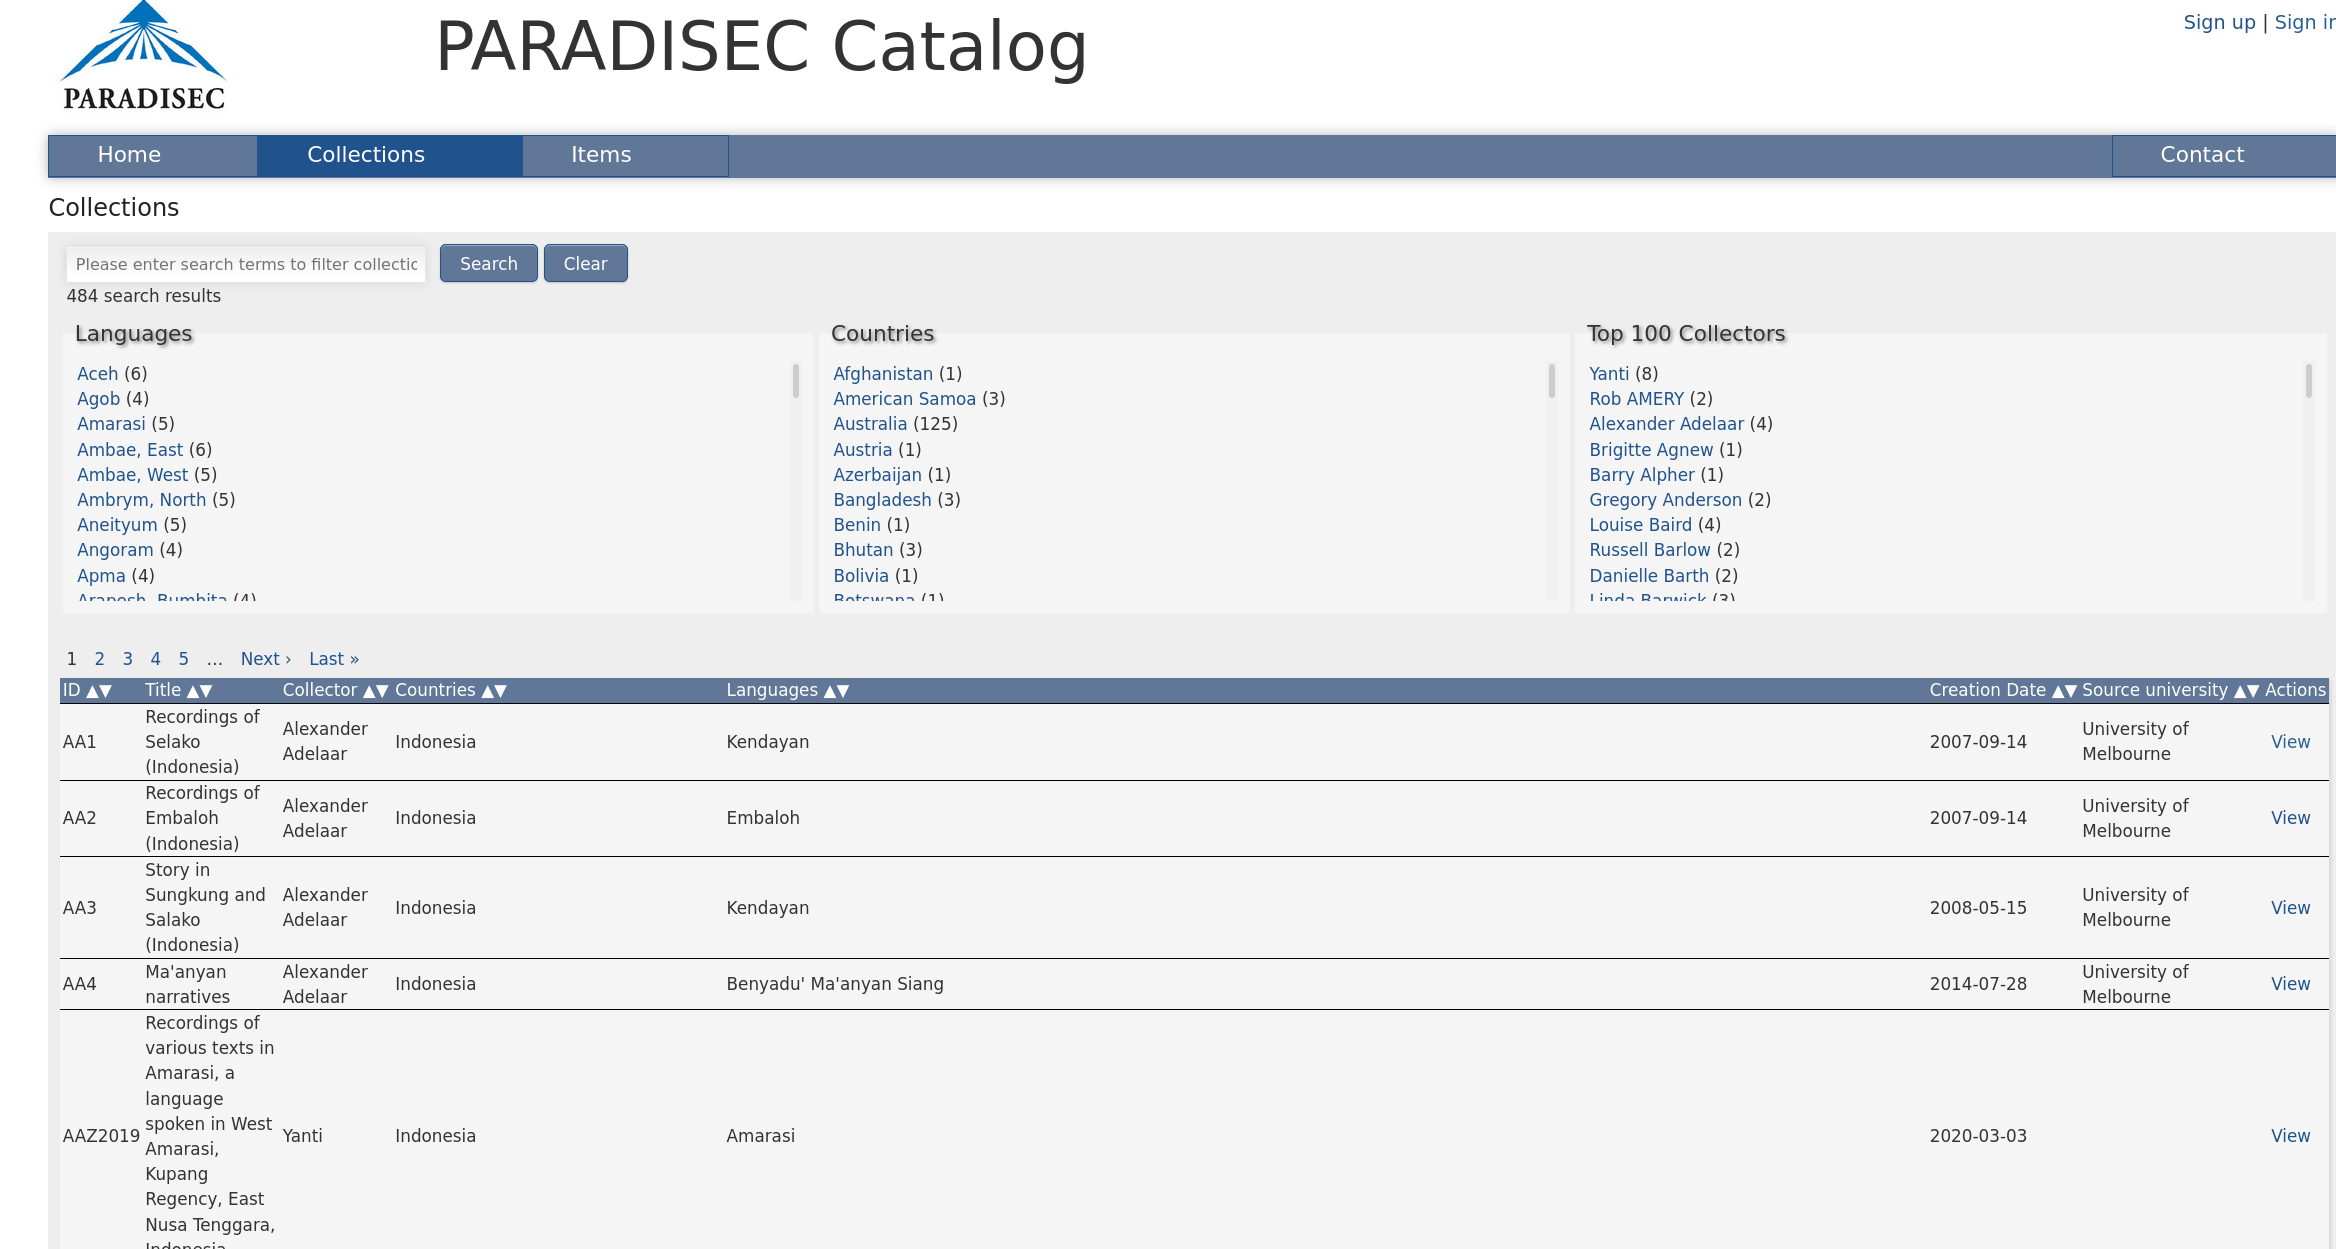
\includegraphics[height=\textheight]{paradisec.png}
}

\frame{
\frametitle{Numerical data}
%   \includegraphics[height=.2\textheight]{./path/to/graphicsfile}
  \begin{itemize}
    \item TROLLing
%     \item figshare
    \item GitHub/GitLab
    \item  Zenodo (also as a general fallback)
    \item GitHub-Zenodo bridge to integrate versioning and archiving
  \end{itemize}
}



\frame{
\frametitle{Trolling}
   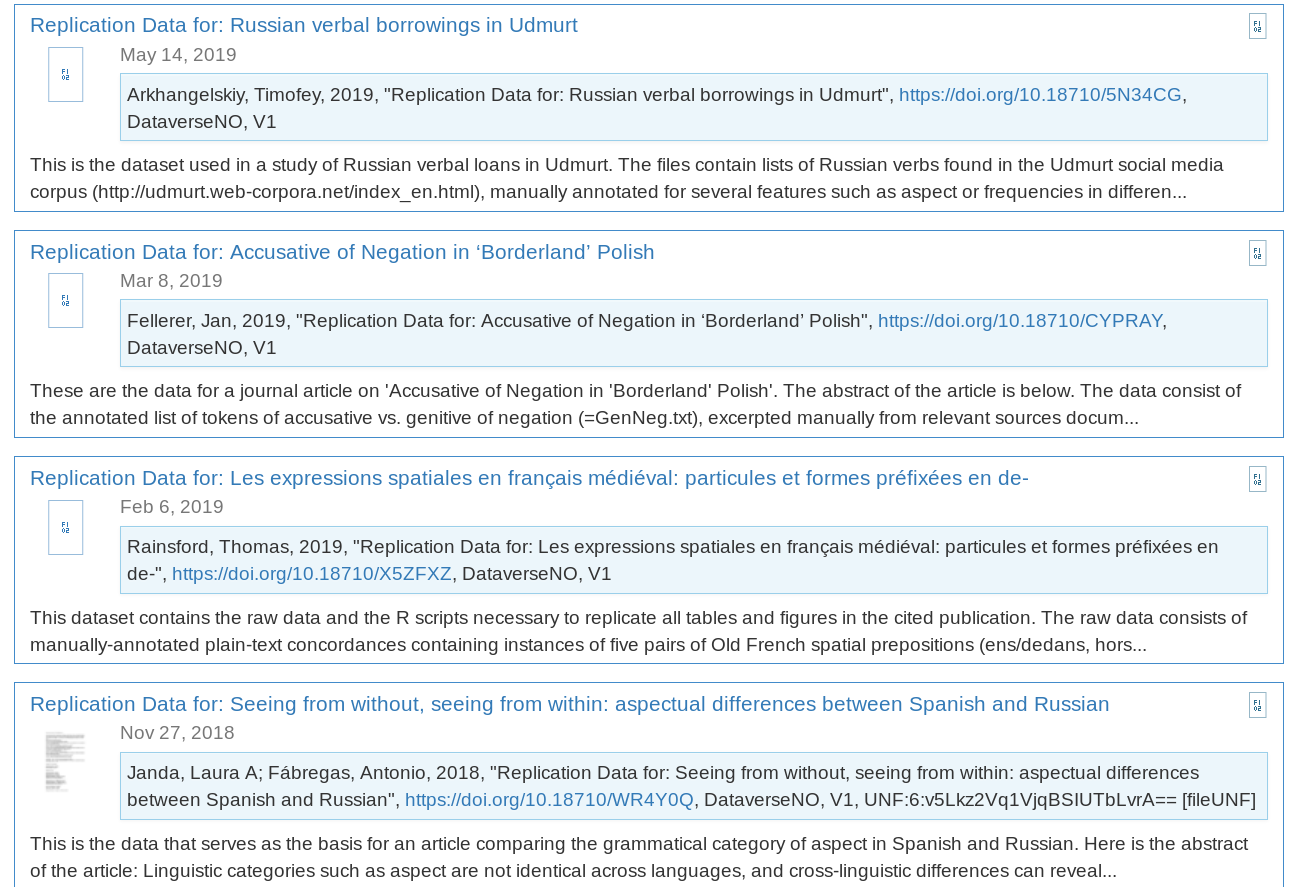
\includegraphics[height=\textheight]{trolling.png}
}


\frame{
\frametitle{Zenodo}
   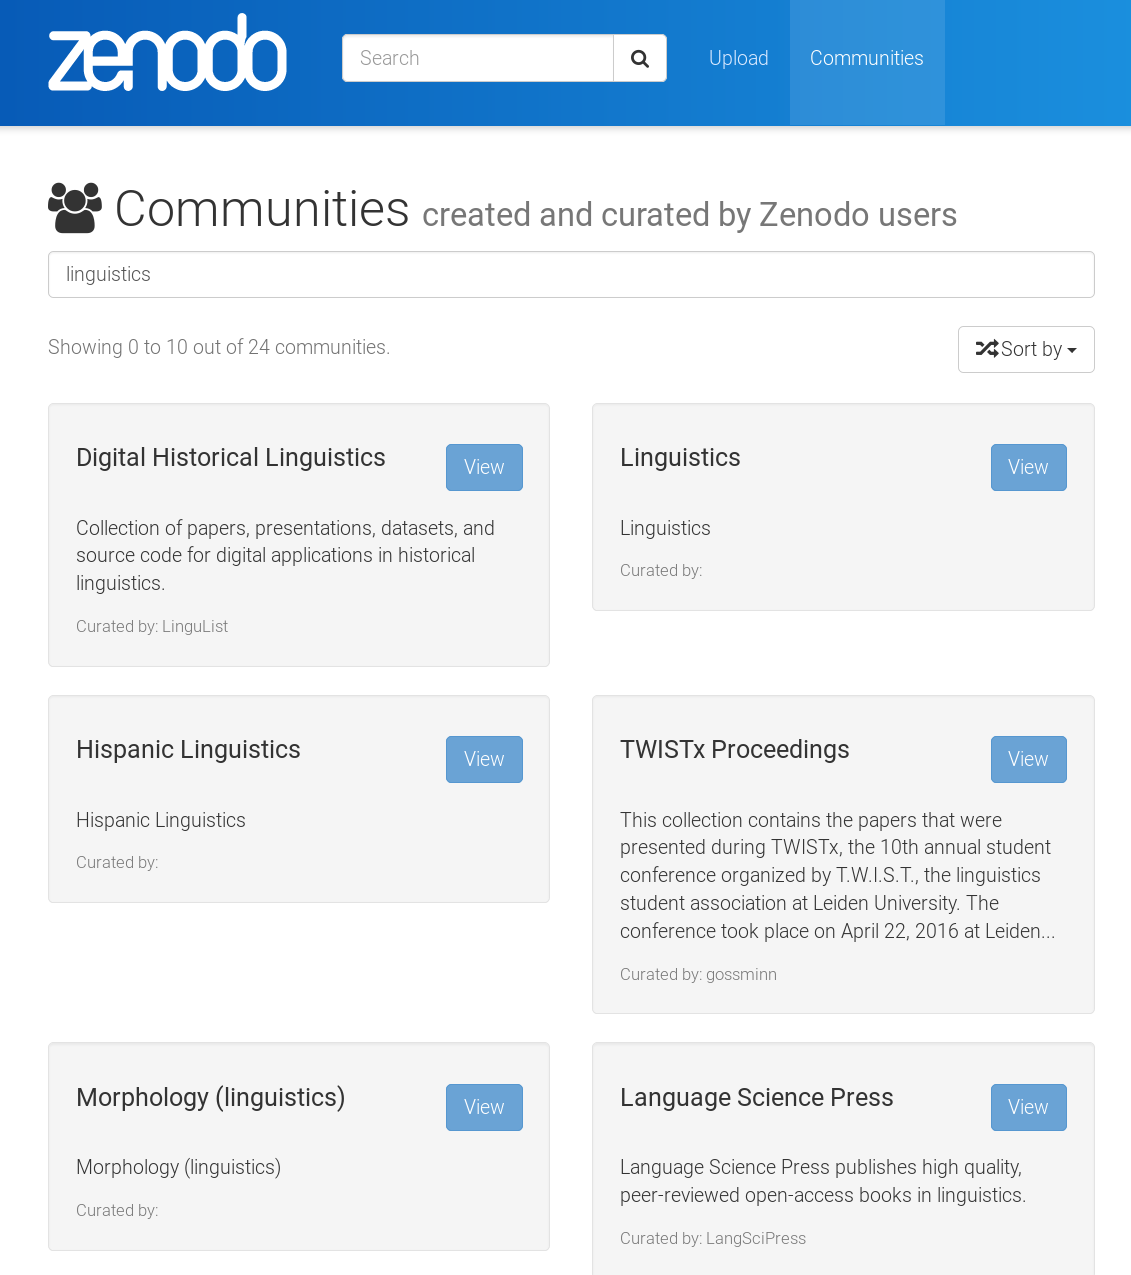
\includegraphics[height=\textheight]{zenodo.png}
}


\frame{
\frametitle{Repositories for texts:\\ Preprint servers}
%   \includegraphics[height=.2\textheight]{./path/to/graphicsfile}
  \begin{itemize}
    \item LingBuzz
    \item semanticsarchive
    \item Rutgers Optimality Archive
  \end{itemize}
}
\frame{
\frametitle{LingBuzz}
   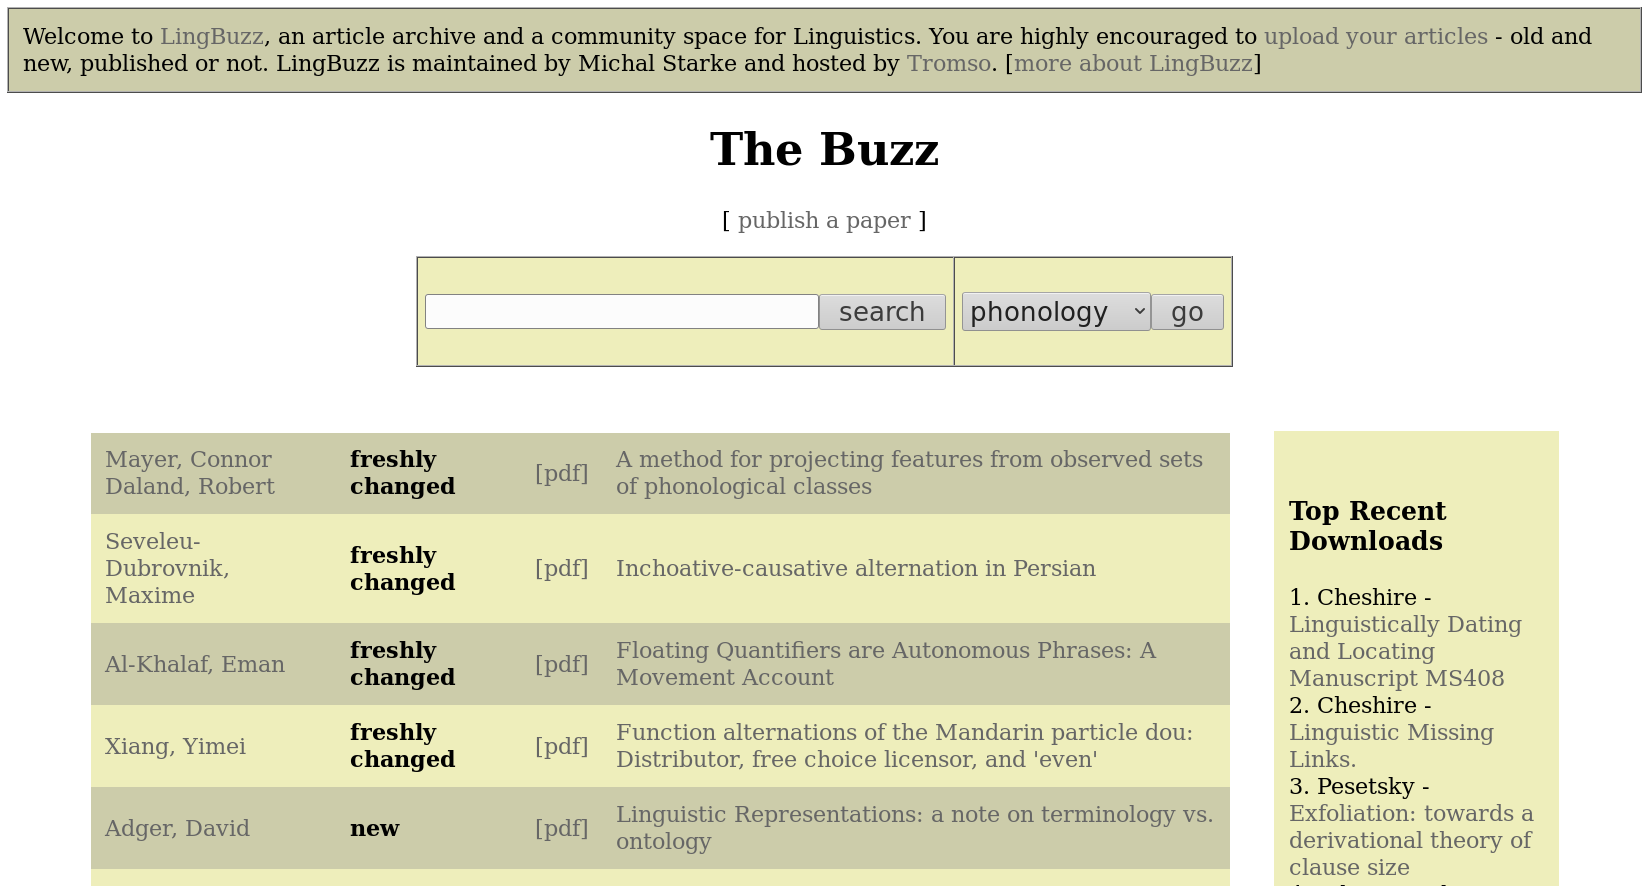
\includegraphics[height=\textheight]{lingbuzz.png}
}

\frame{
\frametitle{semanticsarchive.net}
   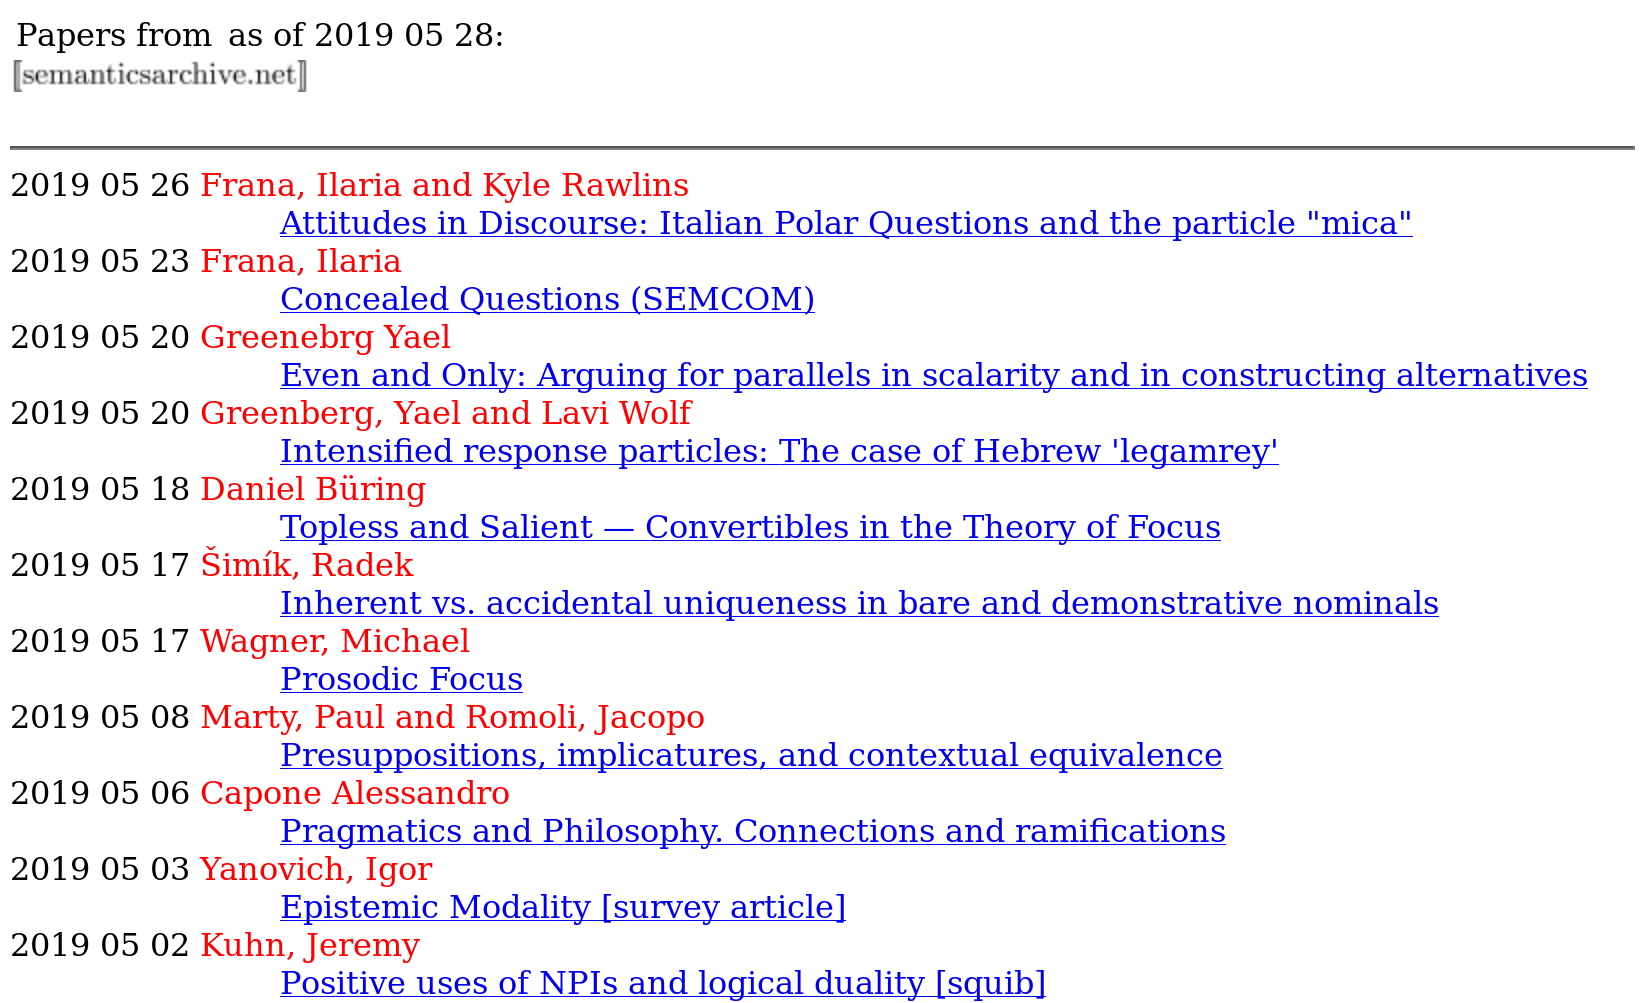
\includegraphics[height=\textheight]{semanticsarchive.png}
}

\frame{
\frametitle{Rutgers Optimality Archive}
   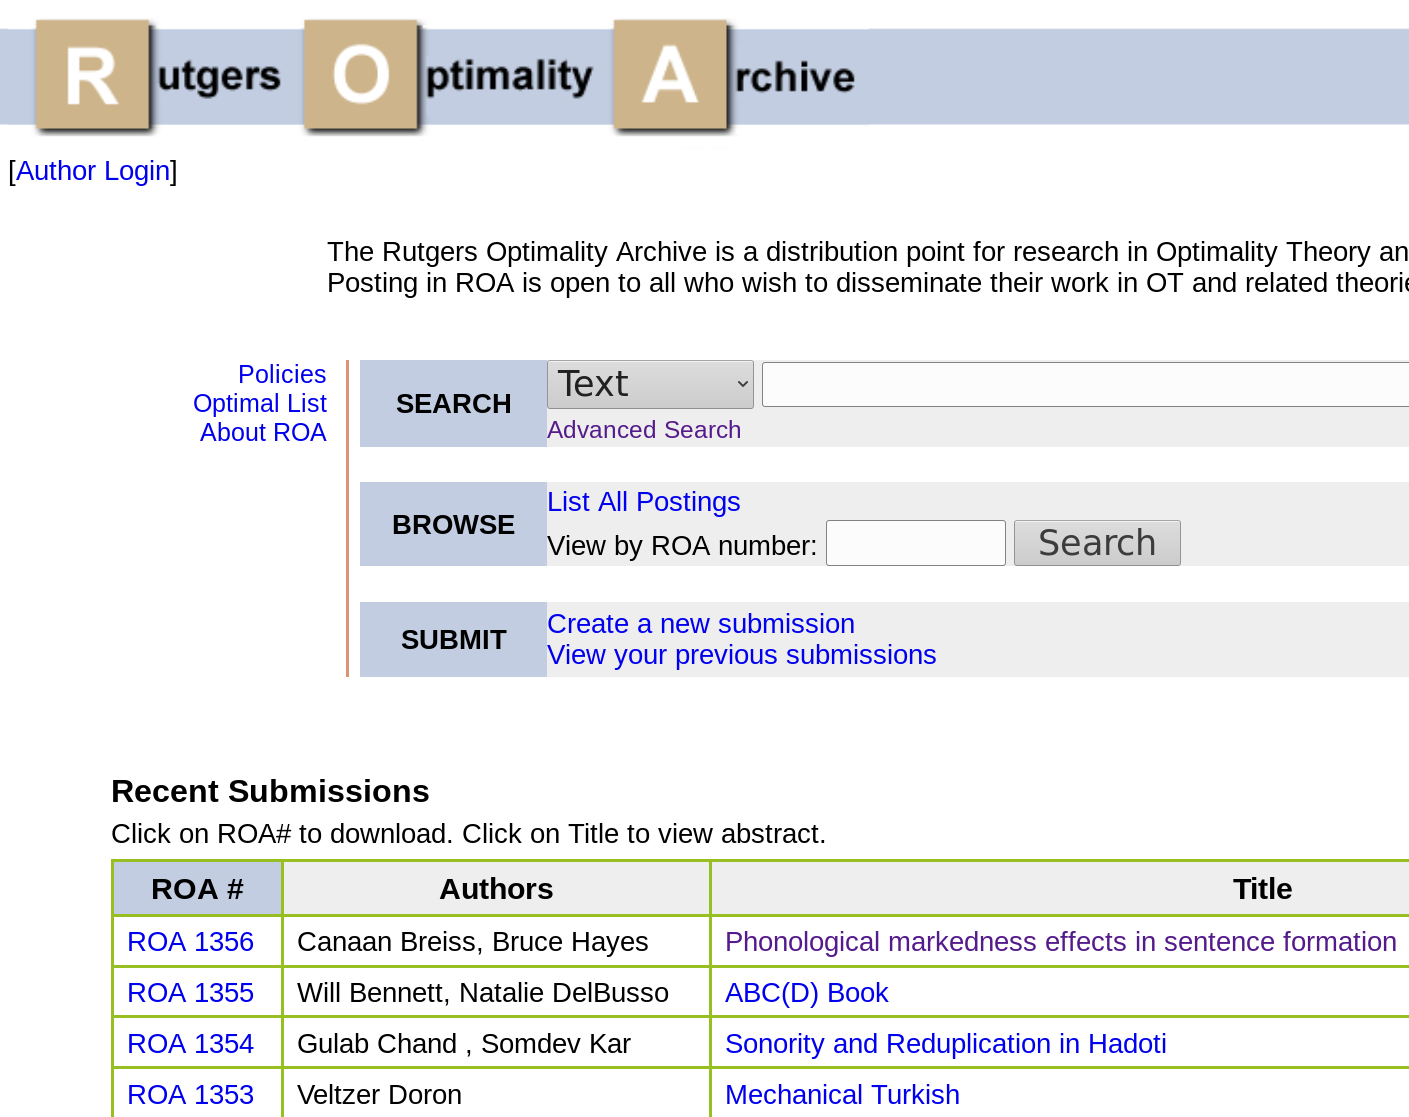
\includegraphics[height=\textheight]{roa.png}
}


\frame{
\frametitle{Academia and Researchgate}
  \begin{itemize}
    \item  Academia.edu and researchgate are NOT repositories
    \item both make money from \textbf{restricting} access
    \end{itemize}
}                    

\frame{
\frametitle{A note on scooping}
  \begin{itemize}
    \item  Scooping means that someone ``steals'' your research while you are still finalising it
    \item that fear is by and large unwarranted 
    \item you can count yourself happy if anybody IS actually interested in your data!
    \item most research actually struggles a lot more with a lack of interest to outsiders rather than scooping 
    \item preprint servers allow you to register your data and establish primacy
  \end{itemize}
}
            
\frame{
\frametitle{And now, finally:\\ publications!}
%   \includegraphics[height=.2\textheight]{./path/to/graphicsfile}
  \begin{itemize}
    \item  raw data + code + write-up = publication
    \item journals
    \item books
    \begin{itemize}
      \item book chapters
    \end{itemize}

  \end{itemize}
}
            

\frame{
\frametitle{Intellectual Property Rights}
%   \includegraphics[height=.2\textheight]{./path/to/graphicsfile}
  \begin{itemize}
    \item  ``Copyright'' in the Anglo-Saxon countries
    \item  ``Urheberrecht/droit d'auteur'' in continental Europe
    \item These are different!
    \item Once you create something, you can decide who can use it and how
    \item Choose wisely and be explicit!
  \end{itemize}
}

\frame{
\frametitle{License}
%   \includegraphics[height=.2\textheight]{./path/to/graphicsfile}
  \begin{itemize}
    \item  Usage rights can be differentiated as follows
    \begin{itemize}
      \item geographical restriction (e.g. \textit{only for France})
      \item type restrictions (e.g. \textit{only for print}) 
      \item exclusive (no-one else has the right) vs. non-exclusive (other people may also get the rights)
      \item copyright transfer agreement (Anglo-Saxon culture)
      \item total buy-out
    \end{itemize}
  \end{itemize}
}

\frame{
\frametitle{Copyright transfer agreement}
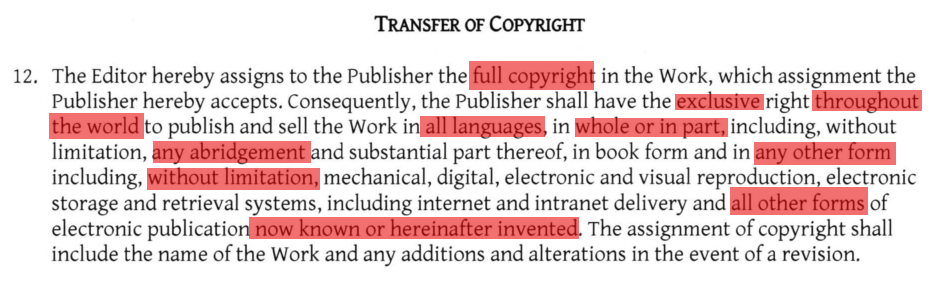
\includegraphics[width=\textwidth]{copyrighttransfer.pdf}
}

\frame{
\frametitle{Contracts}
%   \includegraphics[height=.2\textheight]{./path/to/graphicsfile}
  \begin{itemize}
    \item  Publisher contracts restrict everybody, including yourself 
    \item once you sign away your copyright, you have no longer the right to use your own material 
    \item to reuse tables or graphics in subsequent works of yours, you must first ask the new rights holder for permission 
    \item chasing rights is incredibly annoying
    \item publishers will put your content behind a paywall, meaning that it can actually be more difficult to access once it is officially published than before
    \item publisher vary as to whether and when they allow books to be hosted in repositories  
  \end{itemize}
    }

\frame{
\frametitle{Availability of Nordhoff (ed.) (2012)}
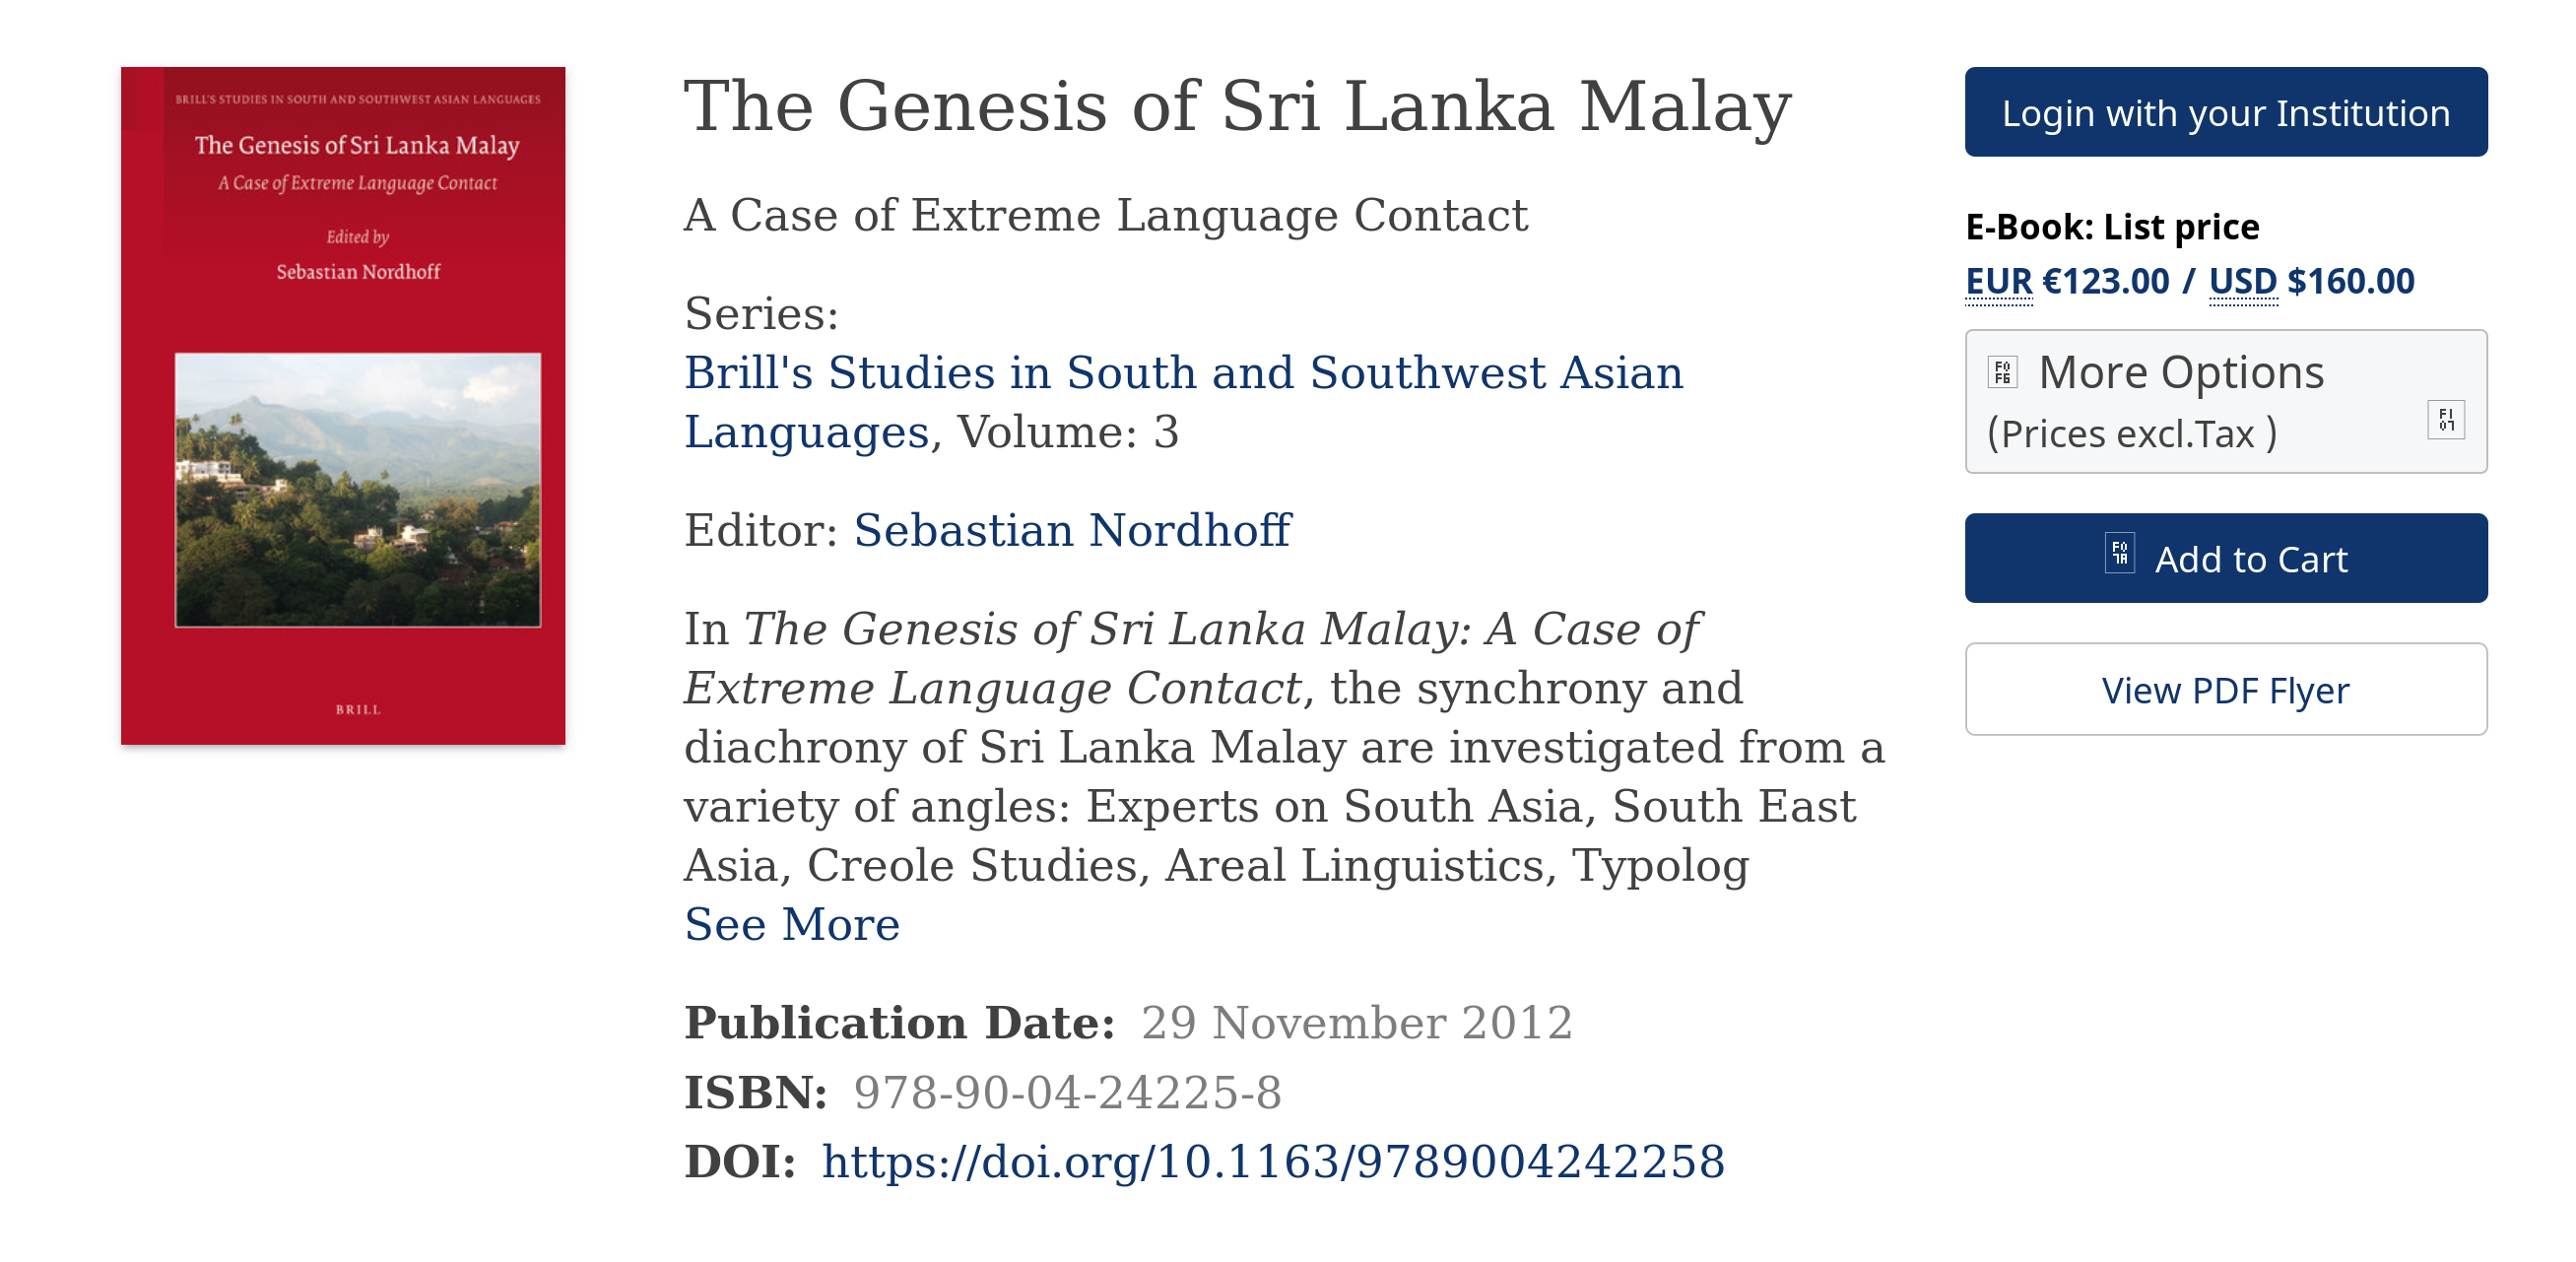
\includegraphics[width=\textwidth]{brillnordhoff.png}
 }

 \frame{
\frametitle{How much money will\\ I make?}
\pause
  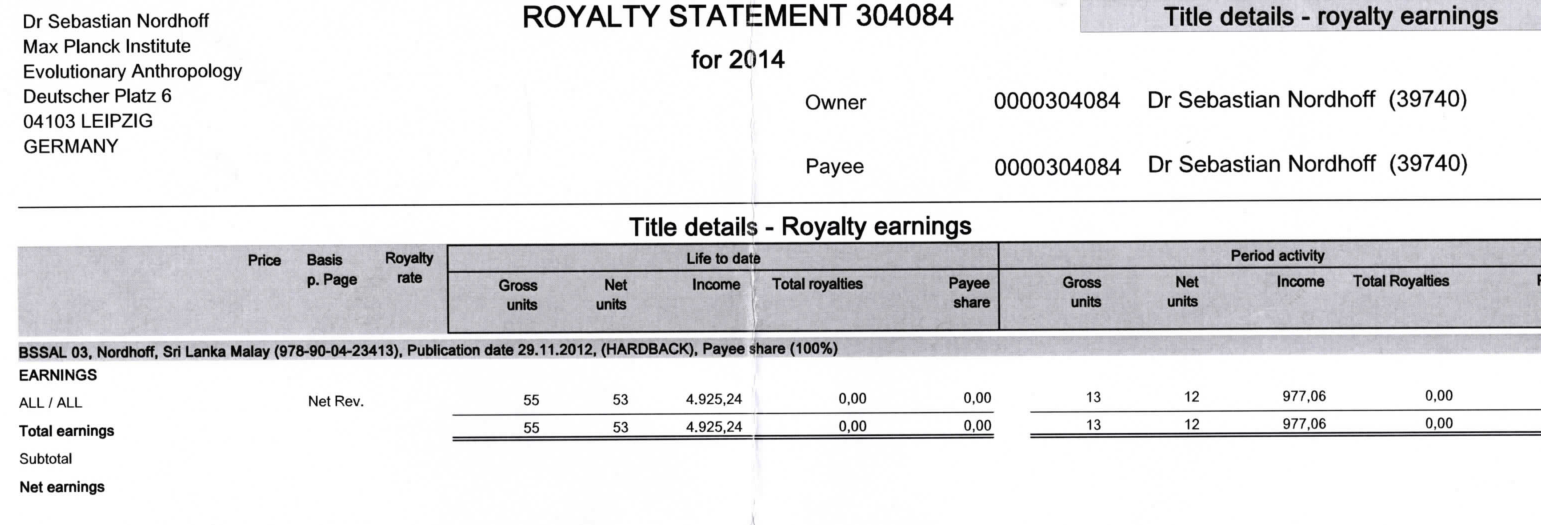
\includegraphics[width=\textwidth]{royalty.pdf}
}

\frame{
\frametitle{Open Access colour codes}
%   \includegraphics[height=.2\textheight]{./path/to/graphicsfile}
  \begin{itemize}
    \item \textbf{green}
    \begin{itemize}
      \item Normal copyrighted publication with a publisher, but copy is archived in an institutional repository
    \end{itemize}
    \item \textbf{gold}
    \begin{itemize}
      \item publication is made openly available against a fee (Article Processing Charge, Book Processing Charge)
    \end{itemize}
    \item \textbf{diamond}
    \begin{itemize}
      \item like Gold OA, but without a fee
    \end{itemize}
      \item (black)
    \begin{itemize}
      \item a copyrighted publication is available via pirate sites/shadow libraries like SciHub or LibGen
    \end{itemize}
    \item (bronze)
    \begin{itemize}
      \item fake open access, not respecting the Berlin Declaration
    \end{itemize}
  \end{itemize}
}


 \frame{
\frametitle{Publisher selection}
%   \includegraphics[height=.2\textheight]{./path/to/graphicsfile}
\begin{itemize}
  \item Fair Open Access Principles (\url{https://www.fairopenaccess.org/the-fair-open-access-principles})
\end{itemize}
\begin{enumerate}
\item    The journal has a \textbf{transparent ownership structure}, and is \textbf{controlled by} and responsive to the \textbf{scholarly community}.
\item     Authors of articles in the journal \textbf{retain copyright}.
\item    All articles are published open access and an \textbf{explicit open access licence} is used.
\item    \textbf{Submission and publication is not conditional} in any way on \textbf{the payment of a fee} from the author or their employing institution, or on membership of an institution or society.
\item    Any \textbf{fees} paid on behalf of the journal to publishers \textbf{are low, transparent, and in proportion} to the work carried out.
\end{enumerate}
}


\frame{
\frametitle{The Green Road:\\ Sherpa Romeo}
%   \includegraphics[height=.2\textheight]{./path/to/graphicsfile}
  \begin{itemize}
    \item Can I deposit my article via the Green Road?
    \item Publisher policies vary
    \begin{itemize}
      \item which version (author submitted version, author accepted manuscript, publisher version)
      \item which embargo period
      \item which repository
    \end{itemize}
    \item Sherpa Romeo is a webservice which gives overviews of different publishers' policies.
    \begin{itemize}
        \item \url{https://v2.sherpa.ac.uk/romeo}
    \end{itemize}
%     \item There is a trick with the Rights Retention Strategy
%     \begin{itemize}
%       \item Before handing in your revised version to the publisher, release it under a Creative Commons license. Then, you  ``re-use'' your own work ``with attribution''. Like that, the copyright does not get transferred.
%     \end{itemize}
  \end{itemize}
}

\frame{
\frametitle{The Golden Road}
%   \includegraphics[height=.2\textheight]{./path/to/graphicsfile}
  \begin{itemize}
    \item Choose your journal
    \item Pay Article processing chargers of 500--3\,000€.
    \begin{itemize}
      \item there might be waivers for people from certain institutions or certain countries
    \end{itemize}
    \item Your article is available as Open  Access
    \item Beware of predatory journals\\
\includegraphics[height=2.5cm]{spam.png}
    \item \url{https://thinkchecksubmit.org}
  \end{itemize}
}


\frame{
\frametitle{Directory of Open Access Books (DOAB)}
  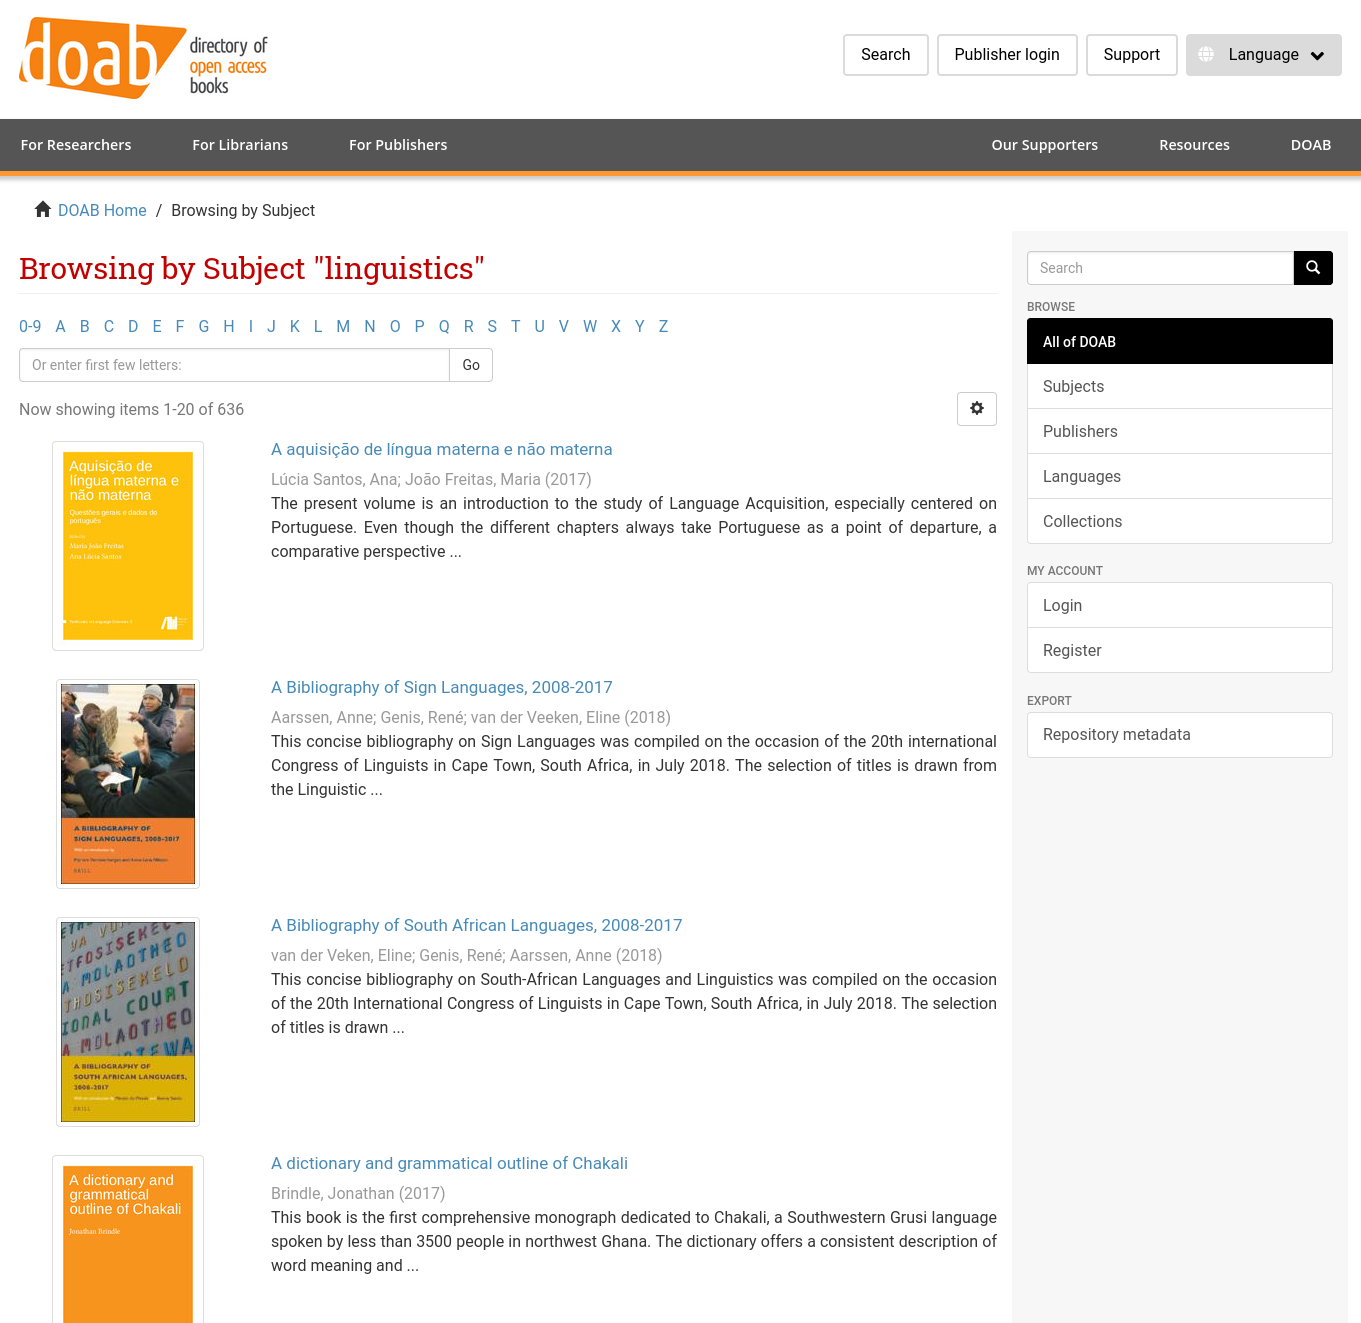
\includegraphics[height=\textheight]{doab.png}
  \begin{itemize}
    \item  \url{https://directory.doabooks.org/browse?type=classification_text&value=linguistics}
  \end{itemize}
}



\frame{
\frametitle{Directory of Open Access Journals (DOAJ)}
  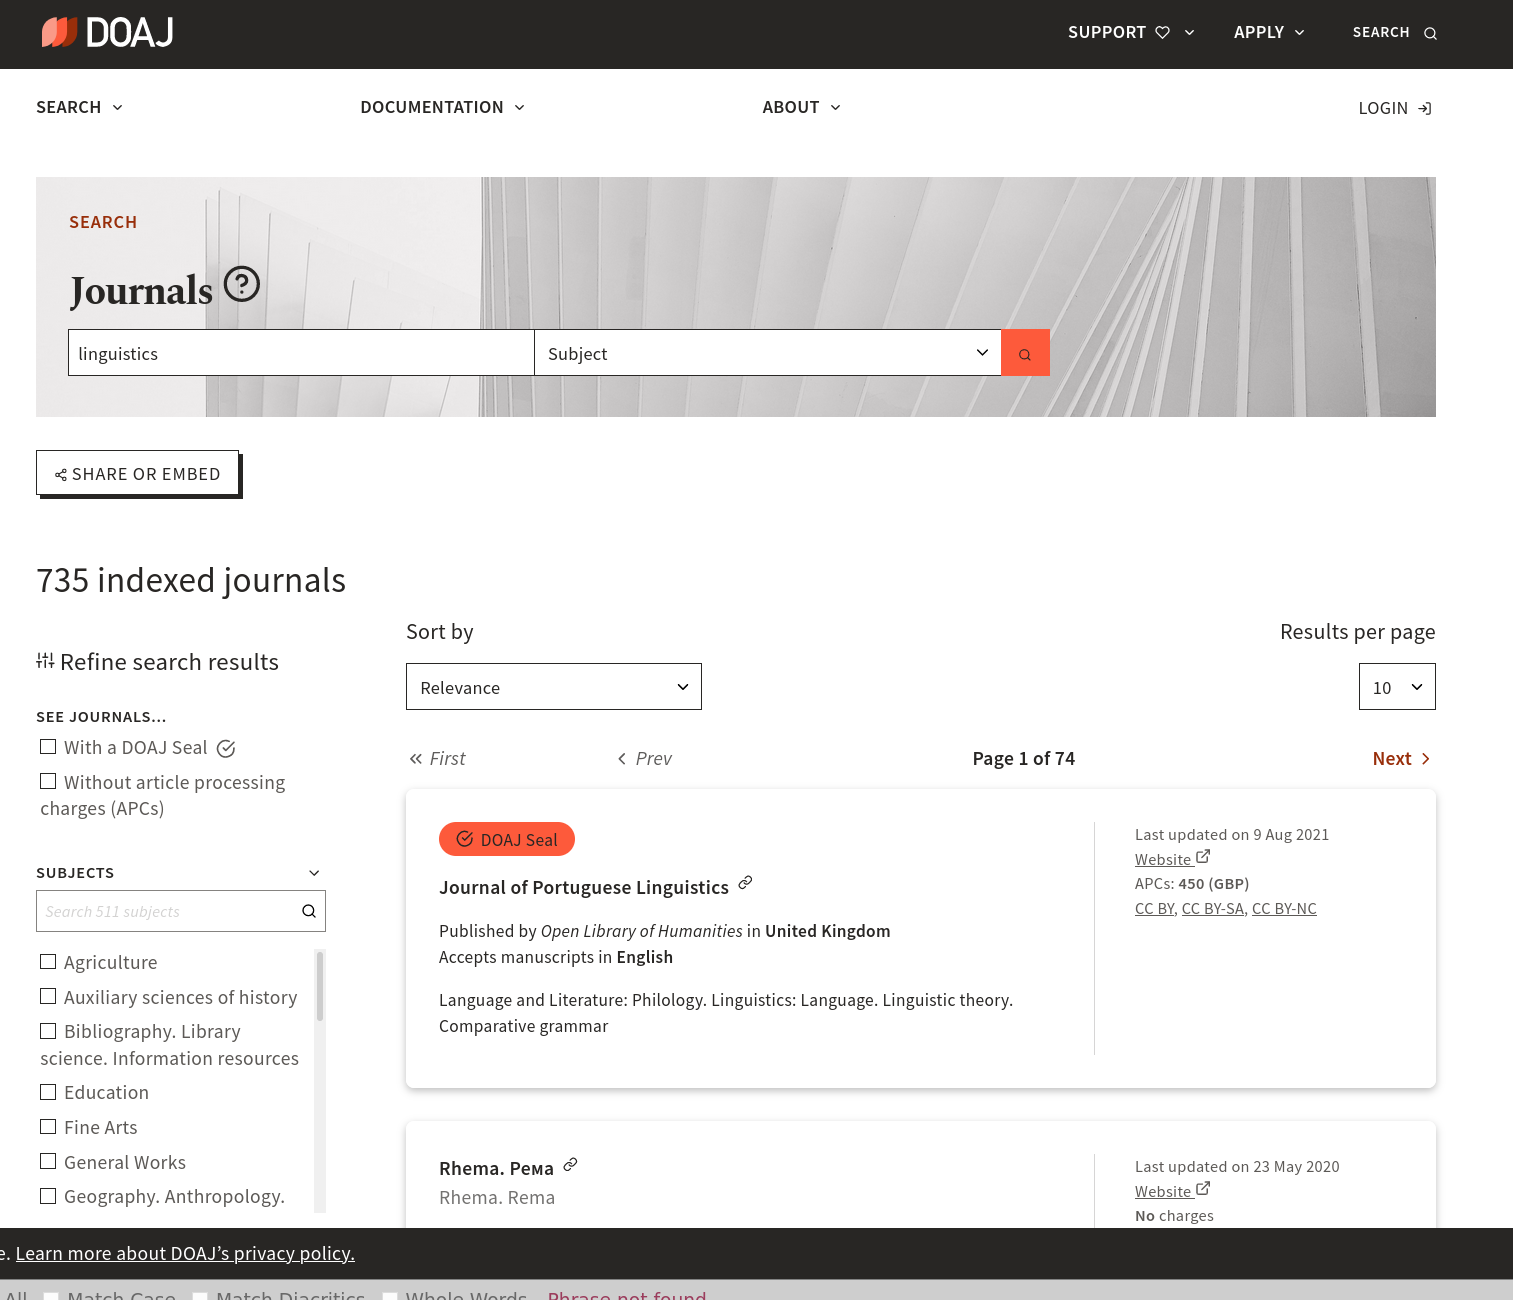
\includegraphics[height=\textheight]{doaj.png}
  \begin{itemize}
    \item  \url{https://directory.doabooks.org/browse?type=classification_text&value=linguistics}
  \end{itemize}
}

\frame{
\frametitle{The Diamond Road}
%   \includegraphics[height=.2\textheight]{./path/to/graphicsfile}
  \begin{itemize}
    \item  Choose your journal
    \item Pay 0€
    \item Your article is available as Open Access
    \item \url{oaling.wordpress.com} has a list of Diamond OA journals in linguistics
  \end{itemize}
}

\frame{
\frametitle{Wrap-up}
%   \includegraphics[height=.2\textheight]{./path/to/graphicsfile}
  \begin{itemize}
    \item  separate your data, scripts, and text
    \item put each of them in dedicated repositories
    \item \textbf{do not sign away your copyright}
    \item choose a CC-BY license
    \item try to go for Diamond OA (also called Platinum)
    \item make a background check for journals and publishers before you submit
  \end{itemize}
}

\frame{
\frametitle{Thank you}
  \includegraphics[width=\textwidth]{nebrija.jpg}
}    

\end{document}
